\documentclass[12pt,preprint]{aastex}

% has to be before amssymb it seems
%\usepackage{color,hyperref}
%\definecolor{linkcolor}{rgb}{0,0,0.5}
%\hypersetup{colorlinks=true,linkcolor=linkcolor,citecolor=linkcolor,
%            filecolor=linkcolor,urlcolor=linkcolor}
%\usepackage{amssymb,amsmath}

\usepackage{color}
\usepackage{url}
\usepackage{graphicx}
\graphicspath{{figures/}}

% For Python code
\usepackage{listings}
\definecolor{lbcolor}{rgb}{0.9,0.9,0.9}
\lstset{language=Python,
        basicstyle=\footnotesize\ttfamily,
        showspaces=false,
        showstringspaces=false,
        tabsize=2,
        breaklines=false,
        breakatwhitespace=true,
        identifierstyle=\ttfamily,
        keywordstyle=\bfseries\color[rgb]{0.133,0.545,0.133},
        commentstyle=\color[rgb]{0.133,0.545,0.133},
        stringstyle=\color[rgb]{0.627,0.126,0.941},
    }

% Draft watermark:
%\usepackage{draftwatermark}
%\SetWatermarkLightness{0.9}
%\SetWatermarkScale{4}

% Some macros
\newcommand{\todo}[1]{{\color{red} [TODO: #1]}}
\newcommand{\foreign}[1]{{\it #1}}

\newcommand{\apriori}{\foreign{a priori}}
\newcommand{\adhoc}{\foreign{ad hoc}}
\newcommand{\etal}{\foreign{et\,al.}}
\newcommand{\etc}{\foreign{etc.}}

\newcommand{\Fig}[1]{Figure~\ref{fig:#1}}
\newcommand{\fig}[1]{\Fig{#1}}
\newcommand{\figlabel}[1]{\label{fig:#1}}
\newcommand{\Eq}[1]{Equation~(\ref{eq:#1})}
\newcommand{\eq}[1]{\Eq{#1}}
\newcommand{\eqlabel}[1]{\label{eq:#1}}
\newcommand{\Sect}[1]{Section~\ref{sect:#1}}
\newcommand{\sect}[1]{\Sect{#1}}
\newcommand{\App}[1]{Appendix~\ref{sect:#1}}
\newcommand{\app}[1]{\App{#1}}
\newcommand{\sectlabel}[1]{\label{sect:#1}}


\begin{document}

\title{Periodograms for Multiband Astronomical Time Series}

\newcommand{\escience}{1}
\newcommand{\uwastro}{2}
\author{Jacob T. VanderPlas\altaffilmark{\escience}}
\author{{\v Z}eljko Ivezi{\'c}\altaffilmark{\uwastro}}
\altaffiltext{\escience}{eScience Institute, University of Washington}
\altaffiltext{\uwastro}{Department of Astronomy, University of Washington}


\begin{abstract}
This paper introduces the {\it multiband periodogram}, a general extension of the standard 
Lomb-Scargle approach for detecting periodic signals in time-domain data. In addition to 
advantanges of the Lomb-Scargle method such as treatment of non-uniform sampling and
heteroscedastic errors, the multiband periodogram significantly improves period finding for randomly 
sampled multiband light curves (e.g., Pan-STARRS, DES and LSST). The light curves in 
each band are modeled as arbitrary truncated Fourier series, with the period and phase 
shared across all bands. The key aspect is the use of Tikhonov regularization which drives
most of the variability into the so-called base model common to all bands, while 
fits for individual bands describe residuals relative to the base model and typically require
lower-order Fourier series. This decrease in the required number of fit parameters is the
main reason for improved performance. We use simulated light curves 
and randomly subsampled SDSS Stripe 82 data to demonstrate the superiority of this 
method compared to other methods from the literature. The Python implementation of 
this method is made publicly available as part of the astroML distribution.
\end{abstract}

\keywords{
    methods: data analysis ---
    methods: statistical
}

\section{Introduction}

Many types of variable stars show periodic flux variability \citep{EM2008}. Periodic variable stars are important 
both for testing models of stellar evolution and for using such stars as distance indicators (e.g., Cepheids 
and RR Lyrae stars). One of the first and main goals of the analysis is to detect variability and to estimate the 
period and its uncertainty. A number of parametric and non-parametric methods have been proposed to 
estimate the period of an astronomical time series \citep[e.g.,][and references therein]{Graham13}.

The most popular non-parametric method is the phase dispersion minimization (PDM) introduced by \cite{PDM1978}. 
Dispersion per bin is computed for binned phased light curves evaluated for a grid of trial periods. The best
period minimizes the dispersion per bin.  A similar and related non-parametric method that has been recently 
gaining popularity is the Supersmoother routine \citep{Reimann94}. It uses a running mean or running linear 
regression on the data to fit the observations as a function of phase to a range of periods. The best period 
minimizes a figure-of-merit, adopted as weighted sum of absolute residuals around the running mean. 
Neither the Supersmoother algorithm nor the PDM method require \apriori{} knowledge of the light curve shape. 
We note that neither method produces posterior probability distribution for the period but rather a single point 
estimate. 

The most popular parametric method is the Lomb-Scargle periodogram, which is discussed in detail in \S~\ref{sec:periodograms}.
The Lomb-Scargle periodogram is related to the $\chi^2$ for a least-square fit of a single sinusoid to data
and can treat non-uniformly sampled time series with heteroscedastic measurement uncertainties. 
The underlying model of the Lomb–Scargle periodogram is nonlinear in frequency and basis functions at different
frequencies are not orthogonal. As a result, the periodogram has many local maxima and thus in practice the global 
maximum of the periodogram is found by grid search \citep[for details see, e.g.][]{ICVG2014}.
A more general parameteric method based on the use of continuous-time autoregressive moving average (CARMA) model
was recently introduced by \citep{Kelly14}. CARMA models can also treat non-uniformly sampled time series with 
heteroscedastic measurement uncertainties, and can handle complex variability patterns. 

A weakness of the above methods is that they require homogeneous measurements -- for astronomy data, this means 
that successive measurements must be taken through a single photometric bandpass (filter). This has not been a major
problem for past surveys because measurements are generally taken through a single photometric filter 
\citep [e.g. LINEAR,][]{LINEAR1}, or nearly-simultaneously in all bands at each observation \citep [e.g. SDSS,][]{Sesar2010}.
For the case of simultaneously taken multiband measurements, \cite{Suveges12} utilized the principal component
method to optimaly extract the best period. Their method is essentially a multiband generalization of the well-known
two-band Welch-Stetson variability index \citep{Stetson1996}. Unfortunately, when data in each band are taken at
different times, the  principal component approach in not applicable. In such cases, past studies have generally relied 
on \adhoc{} methods such as a majority vote among multiple single-band estimates of the 
periodogram \citep[e.g.,][]{Oluseyi12}. 

For surveys that obtain multiband data one band at a time, such as Pan-STARRS \citep{Kaiser2010} and DES \citep{Flaugher08},
and for future multicolor surveys such as LSST \citep{Ivezic08LSST}, this \adhoc{} approach is not optimal. In order to take 
advantage of the full information content in available data, it would be desirable to have a single estimate of the periodogram 
which accounts for all observed data in a manner which is not dependent on the underlying spectrum of the object. 
We propose such a method in this paper. 

The proposed method is essentially a generalization of the Lomb-Scargle method to 
multiband case. The light curves in  each band are modeled as arbitrary truncated Fourier series, 
with the period, and optionally the phase, shared across all bands. The key aspect enabling this approach is the use of Tikhonov regularization 
(discussed in detail in \S \ref{regularization}) which drives most of the variability into the so-called {\it base 
model} common to all bands, while fits for individual bands describe residuals relative to the base model 
and typically require lower-order Fourier series. This decrease in the required number of fit parameters is the
main reason for improved performance. 

\todo{In \S 2, we provide a brief overview of periodograms, including the matrix-based formulation used in this work. In \S... \citet[][hereafter S10]{Sesar2010}...}



\section{Brief Overview of Periodograms \label{sec:periodograms}} 

The detection and quantification of periodicity in time-varying signals is an important area of data analysis within modern time-domain astronomical surveys.
For evenly-spaced data, the {\it Schuster periodogram}, introduced in 1905, gives a quantitative measure of the periodicity of data as a function of the angular frequency $\omega$. For data $\{y_k\}_{k=1}^N$ measured at equal intervals $t_k = t_0 + k\Delta t$, the Schuster periodogram, which measures the spectral power as a function of the angular frequency, is given by
\begin{equation}
  \eqlabel{Schuster}
  C(\omega) = \frac{1}{N}\left| \sum_{k=1}^N y_k e^{i\omega t_k} \right|^2,
\end{equation}
and can be computed very efficiently using the Fast Fourier Transform.

Because astronomical observing cadences are rarely so uniform, many have looked at extending the ideas behind the periodogram to work with unevenly-sampled data. Most famously, \citet{Lomb76} and \citet{Scargle82} extended earlier work to define the {\it normalized periodogram}:
\begin{equation}
  \eqlabel{LombScargle}
  P_N(\omega) = \frac{1}{2\,V}\left[
    \frac{\left[\sum_k(y_k - \bar{y})\cos\omega(t_k - \tau)\right]^2}
    {\sum_k \cos^2\omega(t_k - \tau)}
    +
    \frac{\left[\sum_k(y_k - \bar{y})\sin\omega(t_k - \tau)\right]^2}
    {\sum_k \sin^2\omega(t_k - \tau)}
\right],
\end{equation}
where $\bar{y}$ is the mean and $V$ is the variance of the data $\{y_k\}$, and $\tau$ is the time-offset which makes $P_N(\omega)$ independent of a translation in $t$ \citep[see][for an in-depth discussion]{NumRec}. \citet{Lomb76} showed that this time-offset has a deeper effect: namely, it makes $P_N$ identical to the estimate of harmonic content given a least-squares fit to a single-component sinusoidal model,

\begin{equation}
  \eqlabel{SingleModel}
  d(t) = A\sin(\omega t + \phi).
\end{equation}

This long-recognized connection between spectral power and least squares fitting methods was solidified by \citet{Jaynes87}, who demonstrated that the normalized periodogram of Lomb and Scargle is a sufficient statistic for inferences about a stationary-frequency signal in the presence of Gaussian noise. Building on this result, \citet{Bretthorst88} explored the extension of these methods to more complicated models with multiple frequency terms, nonstationary frequencies, and other more sophisticated models within a Bayesian framework.

While the important features of least squares frequency estimation via Lomb-Scargle periodograms has been discussed elsewhere, we will prevent a brief introduction to the subject in the following section.
The matrix-based formalism we develop here will make clear how the method can be extended to more sophisticated models, including regularized multiband methods.


\section{Background: Matrix Formalism for Periodograms}

In this section we present a quick quantitative introduction to the least squares fitting formulation of the normalized periodogram of \eq{LombScargle}. We denote $N$ observed data points as
\begin{equation}
  D = \{t_k, y_k, \sigma_k\}_{k=1}^N
\end{equation}
where $t_k$ is the time of observation, $y_k$ is the observed value (typically a magnitude), and $\sigma_k$ describes the Gaussian errors on each value. Without loss of generality we will assume that the data $y_k$ are centered such that the measurements within each band satisfy
\begin{equation}
  \eqlabel{ycentered}
  \frac{\sum_k w_ky_k}{\sum_k w_k} = 0
\end{equation}
where the weights are $w_k = \sigma_k^{-2}$.

\subsection{Stationary Sinusoid Model}

The normalized periodogram of \eq{LombScargle} can be derived from the normalized $\chi^2$ of the best-fit single-term stationary sinusoidal model given in \eq{SingleModel}. To make the problem linear, we can re-express the model in terms of the parameter vector $\theta = [A\cos\phi, A\sin\phi]$ so that our model is
\begin{equation}
  \eqlabel{simplemodel}
  y(t|\omega,\theta) = \theta_1\sin(\omega t) + \theta_2\cos(\omega t).
\end{equation}
For a given $\omega$, we can find the maximum likelihood estimate of the parameters $\theta$ by minimizing the $\chi^2$ of the model, which is given by
\begin{equation}
  \chi^2(\omega) = \sum_k \frac{[y_k - y(t_k|\omega,\theta)]^2}{\sigma_k^2}.
\end{equation}
For the single-term Fourier model, it can be shown \citep[See, e.g.][]{ICVG2014} that
\begin{equation}
  \eqlabel{chi2PN}
  \chi_{min}^2(\omega) = \chi^2_0[1 - P_N(\omega)]
\end{equation}
where $P_N(\omega)$ is the normalized periodogram given in \eq{LombScargle} and $\chi^2_0$ is the reference $\chi^2$ for a constant model, which due to the assumption in \eq{ycentered} is simply $\chi^2_0 = \sum_k (y_k/\sigma_k)^2$.


\subsubsection{Matrix Formalism}
The expressions related to the stationary sinusoid model can be expressed more compactly by defining the following matrices:
\begin{equation}
X_\omega = \left[
\begin{array}{cc}
\sin(\omega t_1) & \cos(\omega t_1)\\
\sin(\omega t_2) & \cos(\omega t_2)\\
\vdots & \vdots \\
\sin(\omega t_N) & \cos(\omega t_N)\\
\end{array}
\right];~~
y = \left[
\begin{array}{c}
y_1 \\
y_2\\
\vdots \\
y_N\\
\end{array}
\right];~~
\Sigma = \left[
\begin{array}{cccc}
\sigma_1^2 & 0 &  \cdots & 0\\
0 & \sigma_2^2 &  \cdots & 0\\
\vdots & \vdots &  \ddots & \vdots\\
0 & 0 &  \cdots & \sigma_N^2
\end{array}
\right]
\end{equation}
With these definitions, the model in \eq{simplemodel} can be expressed as a simple linear product, $y(t|\omega,\theta) = X_\omega\theta$, and the model and reference $\chi^2$ can be written

\begin{eqnarray}
  \chi^2(\omega) &=& (y - X_\omega\theta)^T\Sigma^{-1}(y - X_\omega\theta)\\
  \chi^2_0 &=& y^T \Sigma^{-1} y
\end{eqnarray}
The expression for the normalized periodogram can be computed by finding via standard methods the value of $\theta$ which minizes $\chi^2(\omega)$, and plugging the result into \eq{chi2PN}. This yields
\begin{equation}
  \eqlabel{LombScargle2}
  P_N(\omega) = \frac{y^T\Sigma^{-1}X_\omega~[X_\omega^T\Sigma^{-1}X_\omega]^{-1}~X_\omega^T\Sigma^{-1}y}{y^T\Sigma^{-1}y}.
\end{equation}
We note that this expression is equivalent to \eq{LombScargle} in the homoscedastic case with $\Sigma \propto V I$.


\subsubsection{Simple Period Finding}
\sectlabel{simple_period}

\begin{figure}
  \centering
  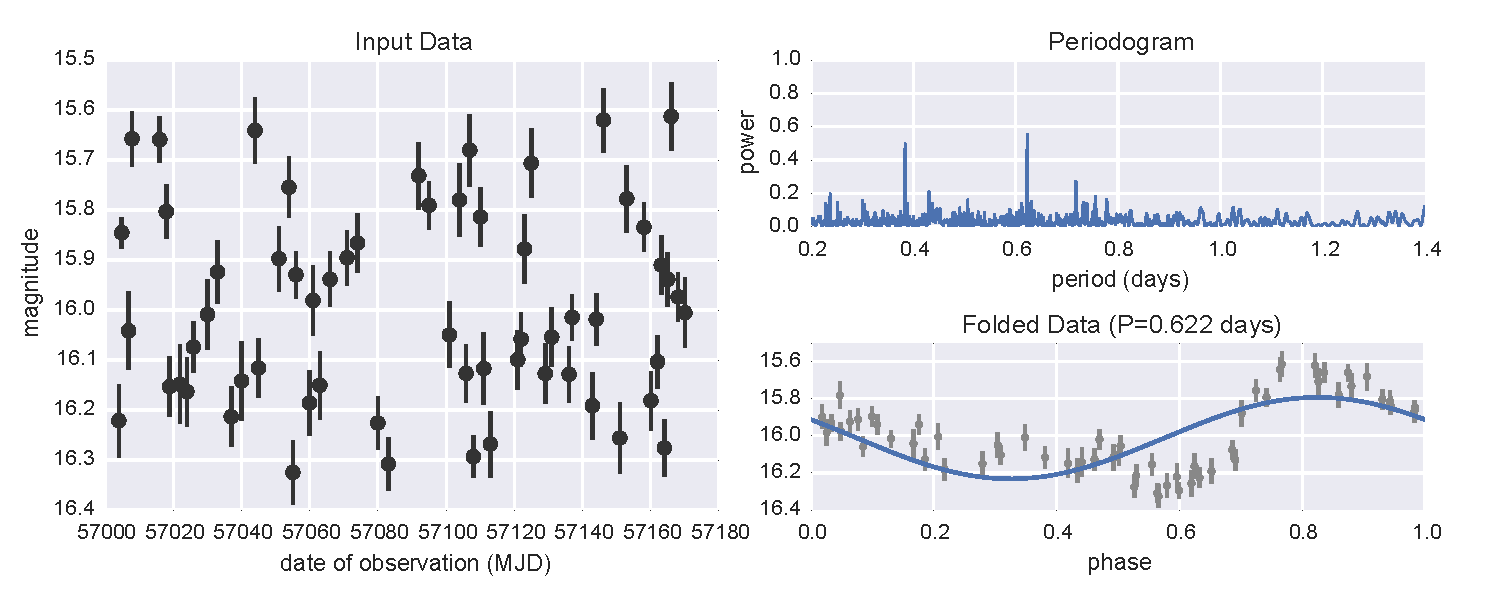
\includegraphics[width=\textwidth]{fig01.pdf}
  \caption{
    An illustration of the basic periodogram and its relationship to the single-term sinusoid model. The left panel shows the input data, while the right panels show the fit derived from the data. The top-right panel shows the periodogram, showing a distinct peak at the true period of 0.622 days, and the bottom-right panel shows the data as a function of phase as defined by this period. Note in the periodogram the presence of the typical aliasing effect, with power located at beat frequencies between the true period and the 1-day observing cadence (see \sect{simple_period} for further discussion).
  }
  \figlabel{basic_example}
\end{figure}

As an example of the standard periodogram in action, we perform a simple single-band harmonic analysis of simulated $r$-band observations of an RR Lyrae light curve, based on empirical templates derived in \citet{Sesar2010} (\fig{basic_example}). The observations are of a star with a period of 0.622 days, and take place on 60 random nights over a 6-month period, as seen in the left panel.

The upper-right panel shows the normalized periodogram for this source as a function of period. While the power does peak at the true period of 0.622 days, an aliasing effect is readily apparent near $P=0.38$. This additional peak is due to beat frequency between the true period $P$ and the observing cadence of $\sim 1$ day. This beat frequency is the first in a large sequence: for nightly observations, we'd expect to find excess power at periods $P_n = P / (1 + nP)$ days, for any integer $n$. The strong alias in \fig{basic_example} corresponds to the $n=1$ beat period $P_n=0.383$. Though it is possible to carefully correct for such aliasing by iteratively removing contributions from the estimated window function \citep[e.g.][]{Roberts87}, we'll ignore this detail in the current work.

The lower-right panel of \fig{basic_example} shows the maximum likelihood interpretation of this periodogram: it is a measure of the normalized $\chi^2$ for a single-term sinusoidal model. Here we visualize the data from the left panel, but folded as a function of phase with the best-fit single-term model over-plot. Here it is apparent that the single-term model is highly biased: RR Lyrae light curves are, in general, much more complicated than a simple sinusoid. Nevertheless, the simplistic sinusoidal model is able to recover the correct frequency to a high degree of accuracy (roughly related to the width of the peak) and significance (roughly related to the height of the peak). For a more complete introduction to and discussion of the single-term normalized periodogram, refer to, e.g. \citet{Bretthorst88} or \citet{ICVG2014}.

\subsection{Extending the Periodogram}
We have shown two forms of the classic normalized periodogram: \eq{LombScargle} and \eq{LombScargle2}. Though the two expressions are equivalent, they each have distinct advantages. The expression in \eq{LombScargle} avoids the explicit construction of a matrix, and thus can be computed very efficiently. Furthermore, through some computational tricks taking advantage of the Fast Fourier Transform, expressions of the form of \eq{LombScargle} can be evaluated exactly for $N$ frequencies in $\mathcal{O}[\log{N}]$ time \citep{Press89}.

The matrix-based formulation of \eq{LombScargle2}, though slower than the Fourier-derived formulation, is a more general expression and allows several advantages:
\begin{enumerate}
  \item It is trivially extended to heteroscedastic and/or correlated measurement noise in the data $y_k$ through appropriate modification of the {\it noise covariance matrix} $\Sigma$
  \item It is trivially extended to more sophisticated linear models by appropriately modifying the {\it design matrix} $X_\omega$.
  \item It is trivially extended to include Tikhonov/L2-regularization terms (see \S \ref{regularization} for more details)  by adding an appropriate diagonal term to the {\it normal matrix} $X_\omega^T\Sigma^{-1}X_\omega$.
\end{enumerate}
In the remainder of this section, we'll explore a few of these modifications and how they affect the periodogram and resulting model fits.


\subsubsection{Stationary Sinusoid with Floating Mean}
\sectlabel{floating_mean}

\begin{figure}
  \centering
  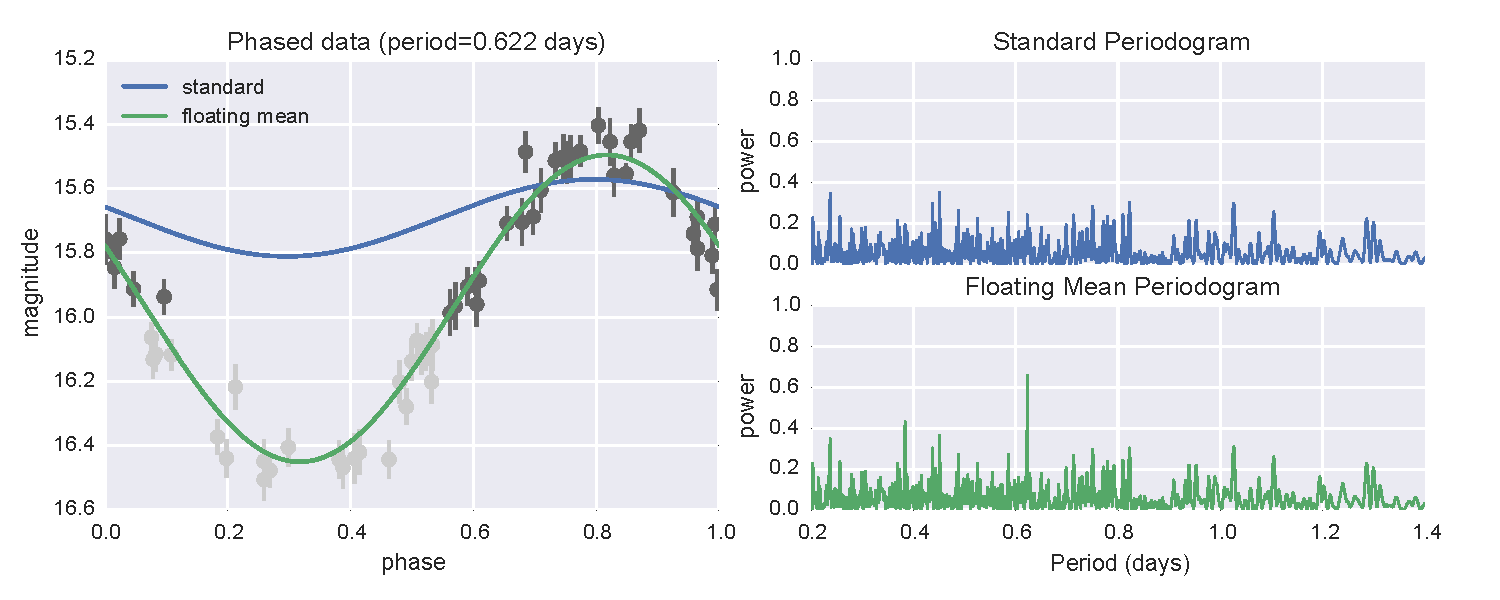
\includegraphics[width=\textwidth]{fig02.pdf}
  \caption{
    An illustration of the effect of the floating mean model for biased data.
    The data consist of 80 observations drawn from a sinusoidal model. To mimick a potentially damaging selection effect, all observations with magnitude fainter than 16 are removed (indicated by the light-gray points). The standard and floating-mean periodograms are computed from the remaining data; these fits are shown over the data in the left panel. Because of this biased observing pattern, the mean of the observed data is not a good predictor of the true mean, and the standard fixed-mean model fails to recover the true period of 0.622 days, while the floating mean model still finds the correct period.
  }
  \figlabel{floating_mean}
\end{figure}

As an example of one of these generalizations, consider the {\it generalized Lomb-Scargle} method of \citet{Zechmeister09}. This adjusts the classic normalized periodogram by allowing the mean of the model to be fit alongside the amplitudes:
\begin{equation}
  y(t~|~\omega, \theta) = \theta_0 + \theta_1\sin\omega t + \theta_2\cos\omega t
\end{equation}
This model can be more accurate than the standard periodogram for certain observing cadences and selection functions. \citet{Zechmeister09} detail the modifications required to the harmonic formalism of \eq{LombScargle} to allow the mean to float in the model. In the matrix formalism, the modification is much more straightforward: all that is required is to add a column of ones to the $X_\omega$ matrix before computing the power via \eq{LombScargle2}.

For well-sampled data, there is usually very little difference between a standard periodogram and a floating-mean periodogram. Where this becomes important is if selection effects or observing cadences cause there to be preferentially more observations at certain phases of the light curve: a toy example demonstrating this situation is shown in \fig{floating_mean}. The data are drawn from a sinusoid with Gaussian errors, and data with a magnitude fainter than 16 are removed to simulate an observational bias (left panel). Because of this observational bias, the mean of the observed data are a poor predictor of the true mean, causing the standard fixed-mean method to poorly fit the data (upper-right panel). The floating-mean approach is able to automatically adjust for this bias, resulting in a periodogram which readily detects the input period of 0.622 days (lower-right panel).


\subsubsection{Truncated Fourier Models}
\sectlabel{multiterm}

\begin{figure}
  \centering
  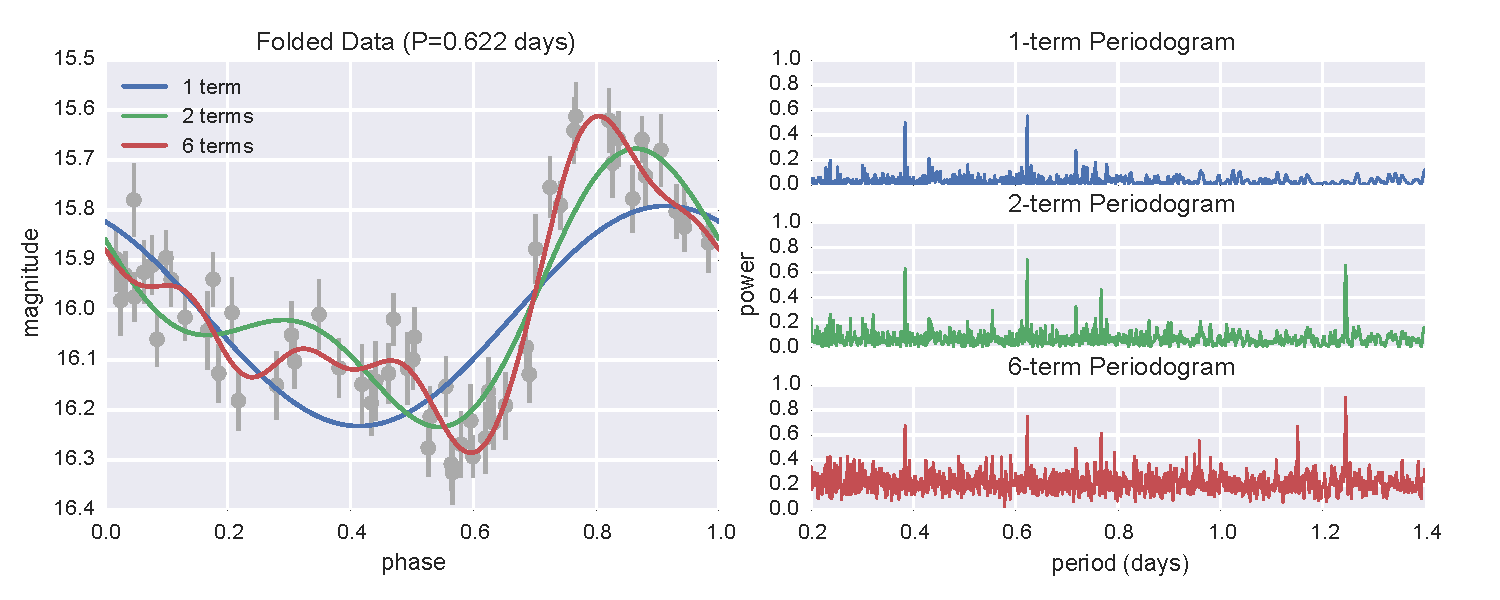
\includegraphics[width=\textwidth]{fig03.pdf}
  \caption{
    An illustration of a periodogram based on several truncated Fourier models.
    The data are the same as those in \fig{basic_example}. Note that the
    higher-order models will generally show periodogram peaks at multiples
    of the true fundamental frequency $P_0$: this is because for integer $n$
    less than the number of Fourier terms in the model, $P_0$ is a higher
    harmonic of the model at $P=nP_0$. Additionally, the increased degrees of
    freedom in the higher-order models let them fit better at any frequency,
    which drives up the ``background'' level in the periodogram.
  }
  \figlabel{multiterm_example}
\end{figure}

As mentioned above, the standard periodogram is equivalent to fitting a single-term stationary sinusoidal model to the data. A natural extension is to instead use a multiple-term sinusoidal model, with frequencies at integer multiples of the fundamental frequency. With $M$ Fourier terms, there are $2M + 1$ free parameters, and the model is given by
\begin{equation}
  y(t|\omega,\theta) = \theta_0 + \sum_{n=1}^M \left[\theta_{2n - 1}\sin(n\omega t) + \theta_{2n}\cos(n\omega t)\right].
\end{equation}
Because this model remains linear in the parameters $\theta$, it can be easily accommodated into the matrix formalism above. For example, an $M = 2$-term floating-mean model can be constructed by building a design matrix $X_\omega$ with $2M + 1 = 5$ columns:
\begin{equation}
X_\omega^{(2)} = \left[
\begin{array}{ccccc}
1 & \sin(\omega t_1) & \cos(\omega t_1) & \sin(2\omega t_1) & \cos(2\omega t_1)\\
1 & \sin(\omega t_2) & \cos(\omega t_2) & \sin(2\omega t_2) & \cos(2\omega t_2)\\
1 & \sin(\omega t_3) & \cos(\omega t_3) & \sin(2\omega t_3) & \cos(2\omega t_3)\\
\vdots & \vdots & \vdots & \vdots & \vdots \\
1 & \sin(\omega t_N) & \cos(\omega t_N) & \sin(2\omega t_N) & \cos(2\omega t_N)\\
\end{array}
\right]
\end{equation}
Computing the power via \eq{LombScargle2} using $X_\omega^{(2)}$ will give the two-term periodogram. As $M$ grows, the size of the design matrix grows, but the periodogram can be computed in the same manner. \fig{multiterm_example} shows a few examples of this multiterm Fourier approach as applied to the simulated RR Lyrae light curve from \fig{basic_example}. There are several important features of this figure that give us insight into the subtleties of this type of multiterm fit.

First, we see in the right panel that all three models show a clear spike at the true period of $P_0 = 0.622$. The higher-order models, however, also show a a spike in power at $P_1 = 2 P_0$: the reason for this is that for and $M>1$-term model, the period $P_0$ is the first harmonic of a model with fundamental frequency $2P_0$, and the higher-order models contain the single-period result.

Second, notice that as the number of terms is increased, the general ``background'' level of the periodogram increases. This is due to the fact that the periodogram power is inversely related to the $\chi^2$ of the fit at each frequency. A more flexible higher-order model can better fit the data at all periods, not just the true period. Thus the observed power of a higher-order Fourier model will be everywhere higher than the power of a lower-order Fourier model.

\subsubsection{Regularized Models \label{regularization}}


\begin{figure}
  \centering
  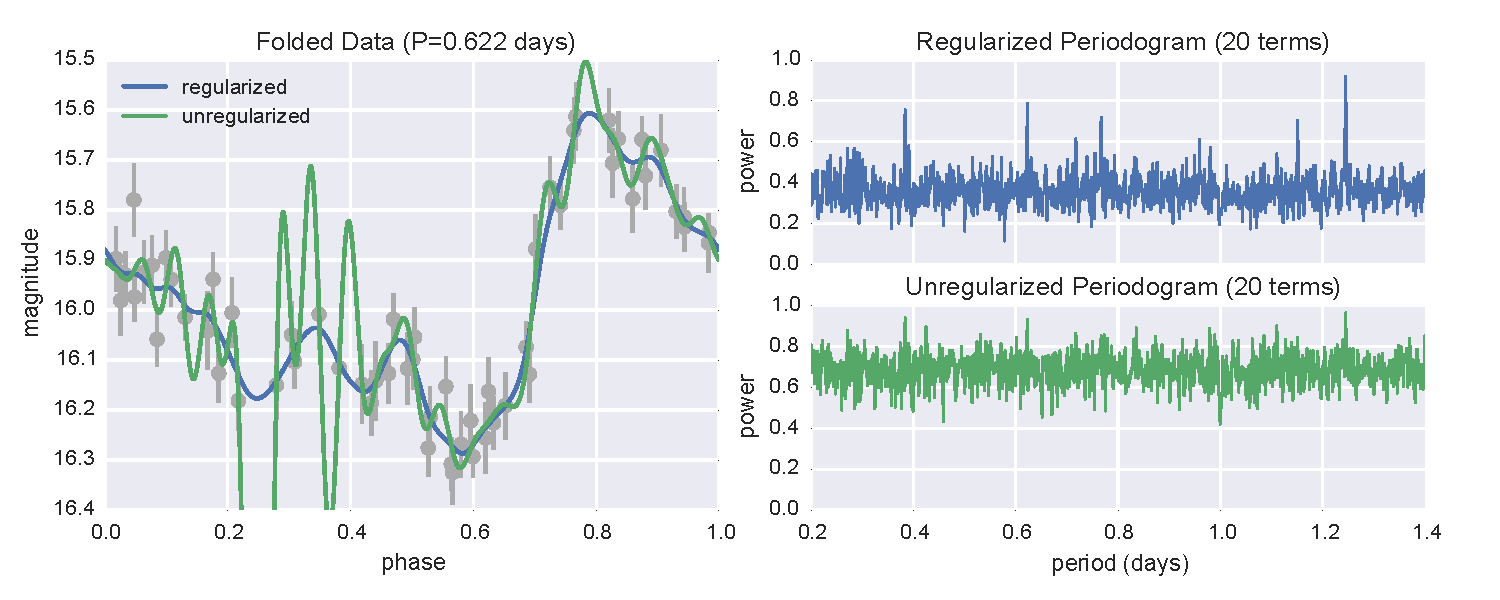
\includegraphics[width=\textwidth]{fig04.pdf}
  \caption{
    The effect of regularization on a high-order model. The data is the same as
    those in \fig{basic_example}. We fit a 20-term truncated Fourier model to
    the data, with and without a regularization term. Without regularization,
    the model oscillates widely to fit the noise in the data. The
    regularization term effectively damps the higher-order Fourier modes and
    removes this oscillating behavior, leading to a more robust model with
    stronger periodogram peaks.
  }
  \figlabel{regularized_example}
\end{figure}

The previous sections raise the question: how complicated a model should we use? We have seen that as we add more terms to the fit, the model will come closer and closer to the observed data. When the number of model parameters equals the number of data points, we can expect to fit the data {\it perfectly} (though in most cases numerical inaccuracies in the fit prevent a truly perfect fit). For very high-order models, such a fit becomes very sensitive to the noise in the data, and we say we have {\it over-fit} the data. This can be addressed by explicitly truncating the series, but we can also use a {\it regularization} term to mathematically ensure a less complicated model.

A regularization term is an explicit penalty on the magnitude of the model parameters $\theta$, and can take a number of forms. For computational simplicity here we'll use an {\it L2 regularization} -- also known as Tikhonov Regularization \citep{Tikhonov1963} or Ridge Regression \citep{Hoerl1970} -- which is a quadratic penalty term in the model parameters added to the $\chi^2$. Mathematically, this is equivalent to the Bayesian approach of using a zero-mean Gaussian prior on the model parameters.

We encode our regularization in the matrix $\Lambda = {\rm diag}([\lambda_1, \lambda_2 \cdots \lambda_M])$ for a model with $M$ parameters, and our expression for ``regularized'' $\chi^2$ becomes
\begin{equation}
  \eqlabel{chi2reg}
  \chi_\Lambda^2(\omega) = (y - X_\omega\theta)^T\Sigma^{-1}(y - X_\omega\theta) + \theta^T\Lambda\theta
\end{equation}
Minimizing this regularized $\chi^2$, solving for $\theta$, and plugging into the expression for $P_N$ gives us the regularized counterpart of \eq{LombScargle2}:
\begin{equation}
  \eqlabel{LombScargleReg}
  P_N(\omega) = \frac{y^T\Sigma^{-1}X_\omega~[X_\omega^T\Sigma^{-1}X_\omega + \Lambda]^{-1}~X_\omega^T\Sigma^{-1}y}{y^T\Sigma^{-1}y}.
\end{equation}
Notice that the effect of this regularization term is to add a diagonal penalty to the normal matrix $X_\omega^T\Sigma^{-1}X_\omega$, which has the additional feature that it can correct ill-posed models where the normal matrix is non-invertible. This feature of the regularization will become important for the multiband models discussed below.

In \fig{regularized_example}, we compare a regularized and unregularized 20-term truncated Fourier model on our simulated RR Lyrae light curve. We use $\lambda = 0$ on the offset term, and make the penalty $\lambda_j$ progressively larger for each harmonic component. The result of the regularized model is less over-fitting to the input data, and a more distinct peaks in the associated periodogram.


\section{A Multiple-Band Model}
\sectlabel{multiband}
To compute a periodogram for multiband data, we'll take advantage of many of the nice features of the matrix form of the normalized periodogram, which easily accommodates arbitrary linear models covering our data.
To account for data in multible bands, we will construct a multi-term Fourier model with the following features:
\begin{enumerate}
  \item An $N_{base}$-term truncated Fourier fit which models a latent parameter, which we'll call the ``overall variability''.
  \item A set of $N_{band}$-term truncated Fourier fits, each of which models the residual of a single band from this overall variability.
\end{enumerate}
The total number of parameters for $K$ filters is then $M_K = (2N_{base} + 1) + K(2N_{band} + 1)$. As a result, for each band $k$ we have the following model of the observed magnitudes:
\begin{eqnarray}
  y_k(t|\omega,\theta) = &\theta_0 + \sum_{n=1}^{M_{base}} \left[\theta_{2n - 1}\sin(n\omega t) + \theta_{2n}\cos(n\omega t)\right]& +\\ 
  &\theta^{(k)}_0 + \sum_{n=1}^{M_{band}} \left[\theta^{(k)}_{2n - 1}\sin(n\omega t) + \theta^{(k)}_{2n}\cos(n\omega t)\right].&
\end{eqnarray}
The important feature of this model is that {\it all bands} share the same base parameters $\theta$, while their offsets $\theta^{(k)}$ are determined individually.

We can construct the normalized periodogram for this model by building a sparse design matrix with $M_K$ columns. Each row corresponds to a single observation through a single band. Columns corresponding to the base model and the matching observation band will have nonzero entries; all other columns will be filled with zeros. For example, the $N_{base}=1$ and $N_{band}=0$ model corresponds to one with a simple single-term periodic base frequency, and an independent constant offset term in each band. The associated design matrix will look as follows:
\begin{equation}
X_\omega^{(1,0)} = \left[
\begin{array}{cccccccc}
1 & \sin(\omega t_1) & \cos(\omega t_1) & 1 & 0 & 0 & 0 & 0\\
1 & \sin(\omega t_2) & \cos(\omega t_2) & 0 & 1 & 0 & 0 & 0\\
1 & \sin(\omega t_3) & \cos(\omega t_3) & 0 & 0 & 0 & 1 & 0\\
\vdots & \vdots & \vdots & & & \vdots & &\\
1 & \sin(\omega t_N) & \cos(\omega t_N) & 0 & 0 & 1 & 0 & 0\\
\end{array}
\right]
\end{equation}
Here the nonzero entries of the final five columns are binary flags indicating the $ugriz$ band of the given observation: in this case, the first row is a $u$-band measurement, the second is a $g$-band, the third is a $i$-band, etc.

On examination of the above matrix, it's clear that the columns are not linearly independent (i.e. $X_\omega$ is low-rank), and thus the parameters of the best-fit model will be degenerate. Intuitively, this is due to the fact that if we add an overall offset to the base model, this can be perfectly accounted for by subtracting that same offset from each of the band columns. Mathematically, the result of this is that the normal matrix $X_\omega^T\Sigma^{-1}X_\omega$ will be non-invertible, and thus the periodogram is ill-defined. In order to proceed, then, we'll either have to use a different model, or use a cleverly-constructed regularization term on one of the offending parameters.

We'll choose the latter here, and regularize all the band columns while leaving the base columns un-regularized: for the above $X_\omega$ matrix, this regularization will look like
\begin{equation}
  \Lambda^{(1,0)} = {\rm diag}([0, 0, 0, \epsilon, \epsilon, \epsilon, \epsilon, \epsilon])
\end{equation}
where $\epsilon$ is some small fraction of the trace of the normal matrix $[X_\omega^T\Sigma^{-1}X_\omega]$. The logic of this choice of regularization is that any component of the model which is common to all bands will be preferentially reflected in the base terms, with independent behavior reflected in the individual band terms. Setting $\epsilon$ to some small fraction of the trace ensures that the regularization effect on the remaining model will be small. With this regularization in place, the model is well-posed and \eq{LombScargleReg} can be used to straightforwardly compute the power. The effective number of free parameters for such a regularized $(N_{base}, N_{band})$ model with $K$ filters is
$M_K^{eff} = 2N_{base}^{eff} + K(2N_{band} + 1)$ where $N_{base}^{eff} = \max(0, N_{base} - N_{band})$ is the effective number of base terms.

The final remaining piece to mention is our assumption in \eq{ycentered} that the data are centered. This is required so that the simple form of the reference $\chi^2_0$ remains valid. For the multiband model, this assumption requires that the data satisfy \eq{ycentered} {\it within each band}: equivalently, we could lift this assumption and compute the reference $\chi^2_0$ of the multiband model with an independent floating mean within each band; the results will be identical.

This multiband approach, then, actually comprises a set of models indexed by their value of $N_{base}$ and $N_{band}$. The most fundamental models have $(N_{base}, N_{band}) = (1,0)$ and $(0,1)$, which we'll call the {\it shared-phase} and {\it multi-phase} models respectively. In the shared-phase model, all variability is assumed to be shared between the bands, with only the fixed offset between them allowed to float. In the multi-phase model, each band has independent variability around a shared fixed offset.

\subsection{Relationship of Multiband and Single-band approaches}
\sectlabel{relationship}
The {\it multi-phase} $N_{base}=0$, $N_{band}=1$ model turns out to be a particularly special case.
The base model is a simple global offset which is degenerate with the offsets in each band, so that the design matrix $X_\omega$ can be straightforwardly rearranged as block-diagonal. A block-diagonal design matrix in a linear model indicates that components of the model are being solved independently: here these independent components amount to the single-band floating-mean model from \sect{floating_mean}, fit independently within each of the $K$ bands. This particular multiband model can give us insight into the relationship between single-band and multiband approaches.

For band $k$, we'll denote the single-band floating-mean periodogram as
\begin{equation}
  P_N^{(k)}(\omega) = 1 - \frac{\chi^2_{min, k}(\omega)}{\chi^2_{0,k}}
\end{equation}
The full multiband periodogram is given by
\begin{equation}
  P_N^{(0,1)}(\omega) = 1 - \frac{\sum_{k=1}^K\chi^2_{min, k}(\omega)}{\sum_{k=1}^K\chi^2_{0,k}}
\end{equation}
and it can easily be shown that the $P_N$ can be constructed as a weighted sum of $P_N^{(k)}$:
\begin{equation}
  P_N^{(0,1)}(\omega) = \frac{\sum_{k=1}^K\chi^2_{0,k}P_N^{(k)}}{\sum_{k=1}^K\chi^2_{0,k}}.
\end{equation}
This tells us how we can construct a particular case of the multi-term periodogram from a weighted sum of periodograms in each band, where the weights $\chi^2_{0,k}$ reflect both the number of measurements in each band and how much those measurements deviate from a simple constant reference model.

\subsection{Multiband Periodogram for Simulated Data}
\sectlabel{Simulated}

\begin{figure}
  \centering
  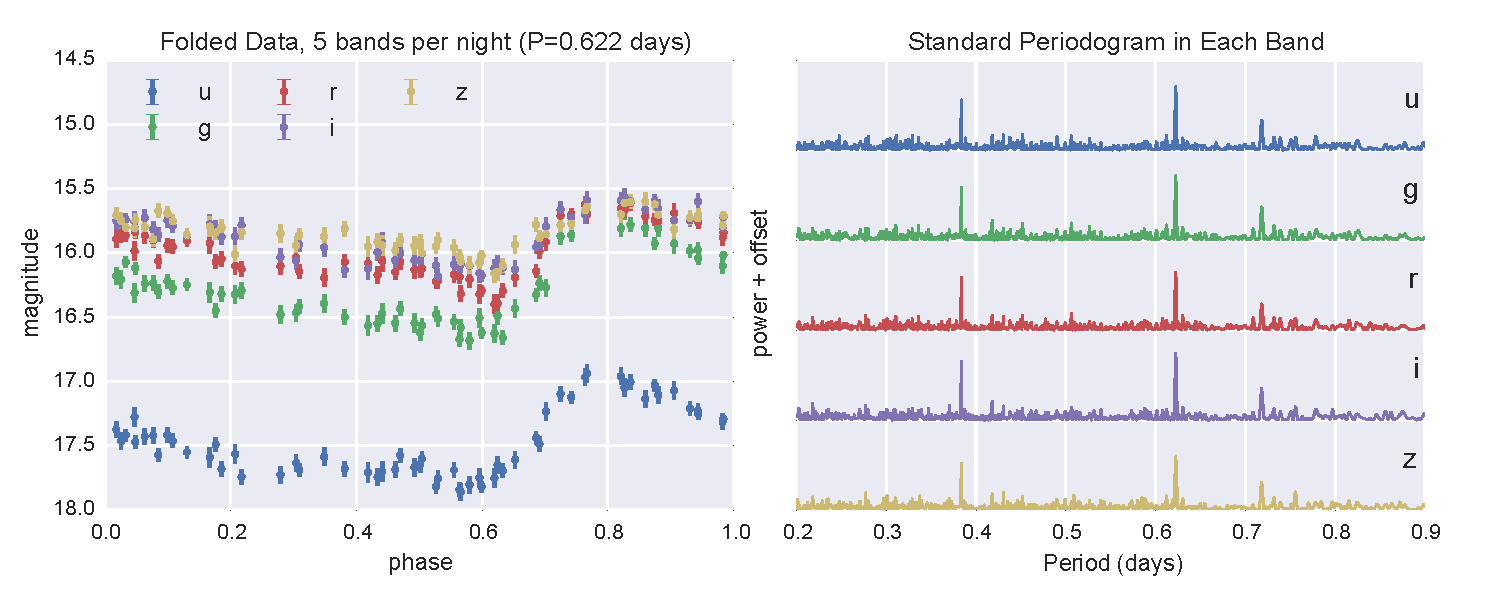
\includegraphics[width=\textwidth]{fig05a.pdf}
  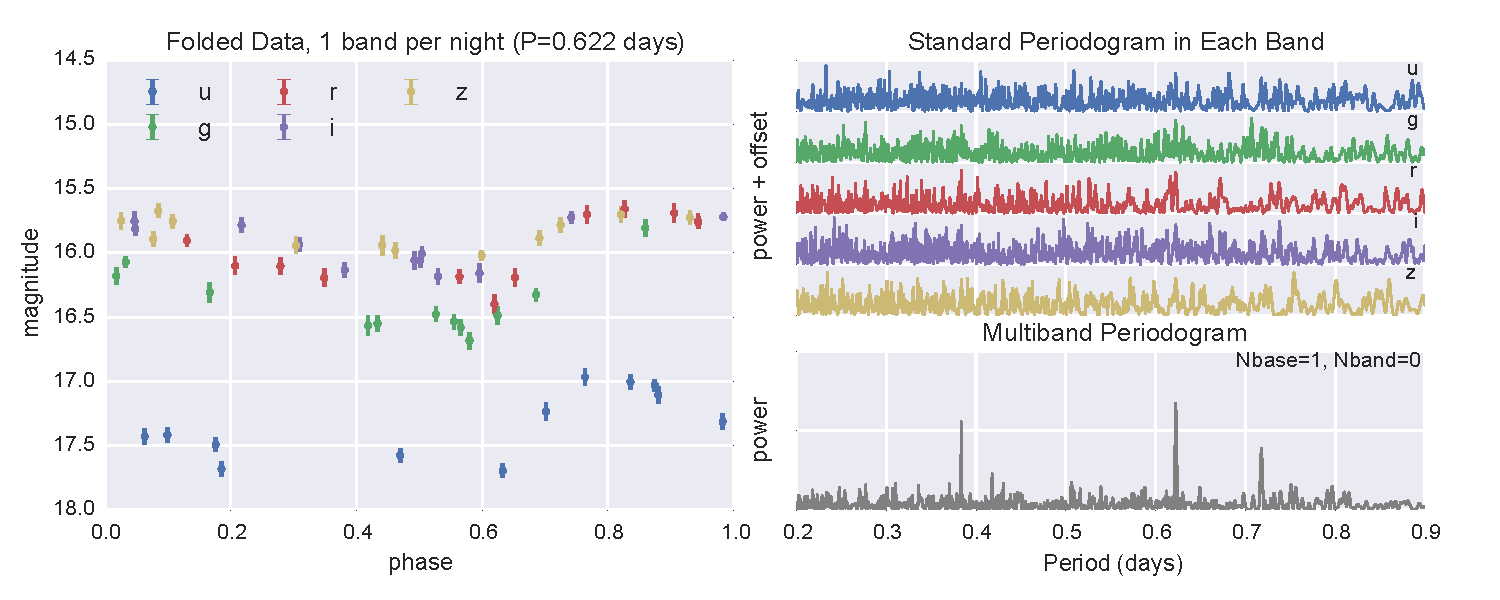
\includegraphics[width=\textwidth]{fig05b.pdf}
  \caption{
    An illustration of the performance of the multiband periodogram. The
    upper panels show simulated $ugriz$ observations of an RR Lyrae light
    curve in which all 5 bands are observed each night. With 60 observations
    in each band, a periodogram computed from any single band is sufficient to
    determine the true period of 0.622 days. The lower panels show the same
    data, except with only a single $ugriz$ band observed each night (i.e.
    12 observations per band). In this case, no single band has enough
    information to detect the period. The shared-phase multiband approach
    of \sect{multiband} (lower-right panel) combines the information from
    all five bands, and results in a significant detection of the true period.
  }
  \figlabel{multiband_sim}
\end{figure}

\begin{figure}
  \centering
  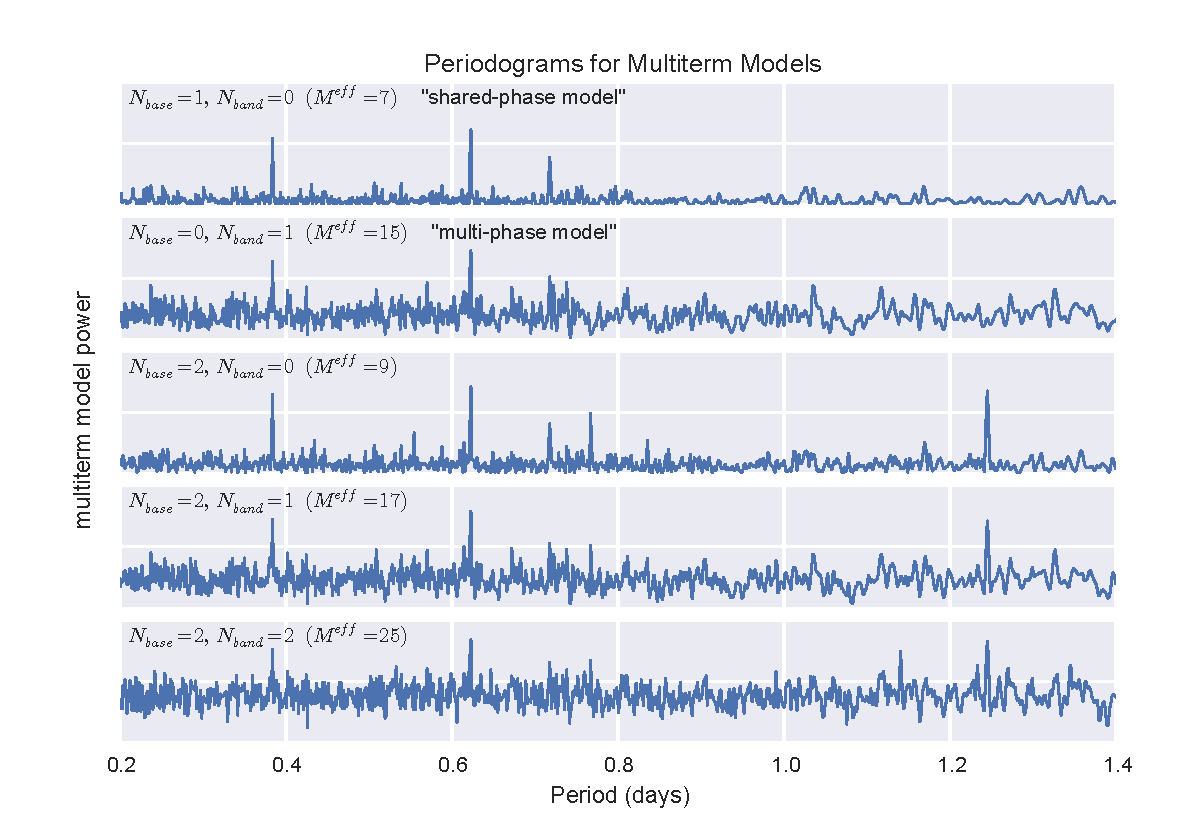
\includegraphics[width=0.8\textwidth]{fig06.pdf}
  \caption{
    Comparison of the periodograms produced by various multiband models.
    The data is the same as that used in \fig{multiband_sim}. $N_{base}$ gives
    the number of Fourier terms in the base model, and $N_{band}$ gives the
    number of Fourier terms used to fit the residuals around this model within
    each band. The characteristics discussed with previous figures are also
    seen here: in particular, the level of ``background noise'' in the
    periodogram grows with the model complexity $M$,
  } 
  \figlabel{multiband_models}
\end{figure}

Before applying the multiband method to real data, let's explore its effectiveness on a simulated RR Lyrae lightcurve.
The upper panels of \fig{multiband_sim} show a multiband version of the simulated RR Lyrae light curve from \fig{basic_example}.
The upper-right panel shows 60 nights of observations spread over a 6-month period, and for each night all five bands ({\it u,g,r,i,z}) are recorded.
Using the typical approach from the literature prior to this paper, we individually compute the standard normalized periodogram within each band: the results are shown in the upper-right panel.
Here the data is well-enough sampled that a distinct period of 0.622 days can be recognized within each individual band, up to the aliasing effect discussed in \sect{simple_period}.
Previous studies have made use of the information in multiple bands to choose between aliases and estimate uncertainties in determined periods \citep[e.g.][]{Oluseyi12,Sesar2010}.
While this approach is sufficient for well-sampled data, it becomes problematic when the multiband data is more sparsely sampled.

The lower panels of \fig{multiband_sim} show the same 60 nights of data, except with only a {\it single} band observation recorded each night. The lower-left panel shows the observations as a function of phase, and the lower-right panels show the periodograms derived from the data. With only 12 observations for each indiviudal band, it is clear that there is not enough data to accurately determine the period within each single band. The shared-phase multiband approach (i.e. $(N_{base},N_{band})=(1,0)$), shown in the lower-right panel, makes use of all the information in a single model, and clearly recovers the true frequency of 0.622 days.

This shared-phase $(1,0)$ model is only one of the possible multiband options, however: \fig{multiband_models} shows multiband fits to this data for models with various combinations of $(N_{base},N_{band})$. We see here many of the characteristics noted above for single-band models: as discussed in \sect{multiterm}, increasing the number of Fourier terms leads to power at multiples of the fundamental period. Additionally, increasing the model complexity (roughly indexed by the effective number of free parameters $M^{eff}$) tends to increase the background level of the periodogram, potentially obscuring significant peaks. For this reason, models with $N_{base} > N_{band}$ are the most promising: they allow a flexible fit with minimal model complexity.

Below, we'll apply the simplest of this class of models, the $(1, 0)$ shared-phase model, to data from the Stripe 82 of the Sloan Digital Sky Survey.


\section{Application to Stripe 82 RR Lyrae}

Stripe 82 is a three hundred square degree equatorial region of the sky which was repeatedly imaged through multiple band-passes during the second phase of the Sloan Digital Sky Survey (SDSS II).
As a real-world test of the multiband periodogram method, we consider the SDSS-2 observations of 483 RR Lyrae stars compiled and studied by S10.
S10 determined periods for these stars based on an emperically-derived light curve templates. Because the template-fitting method is extremely computationally intensive, S10 first determined candidate periods by taking the top 5 results of the supersmoother \citep{Reimann94} algorithm applied to the $g$-band; template fits were then performed at each candidate period and the period with the best template fit was reported as the true period. In this section, we make use of this dataset to quantitatively evaluate the effectiveness of the multiband periodogram approach in the case of this real-world data.

\subsection{Densely-sampled Multiband Data}

\begin{figure}
  \centering
  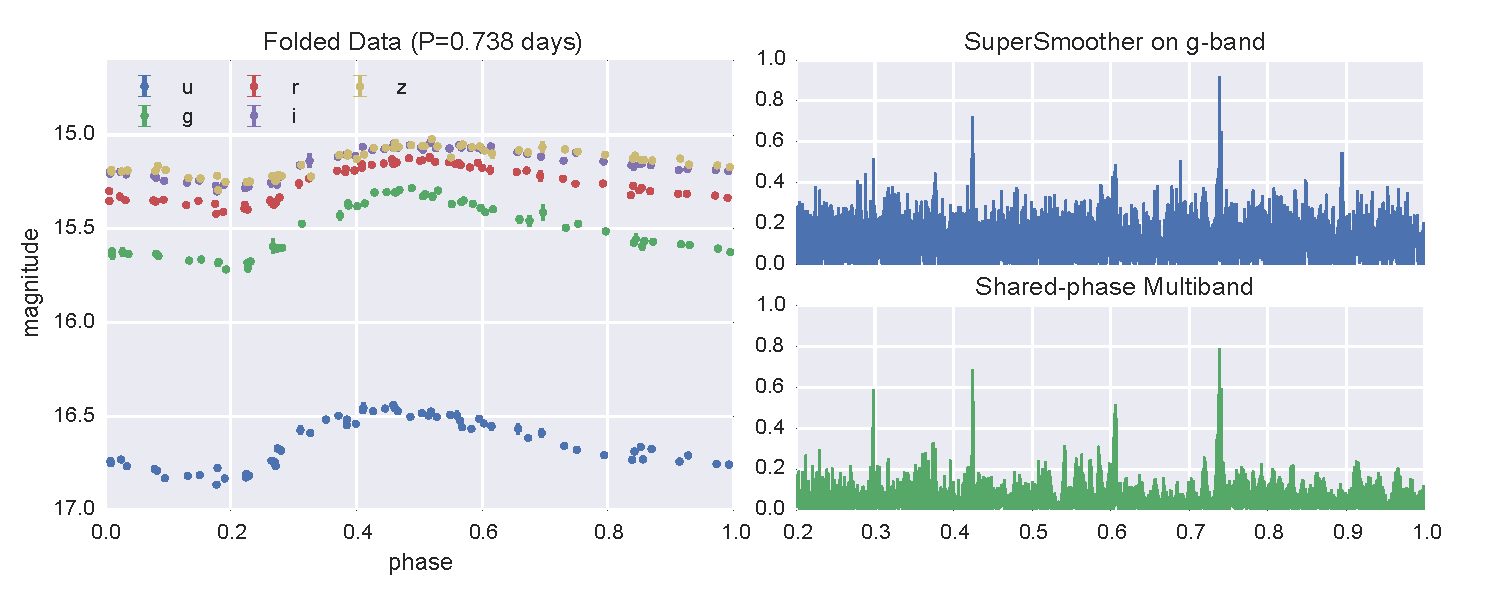
\includegraphics[width=\textwidth]{fig07a.pdf}
  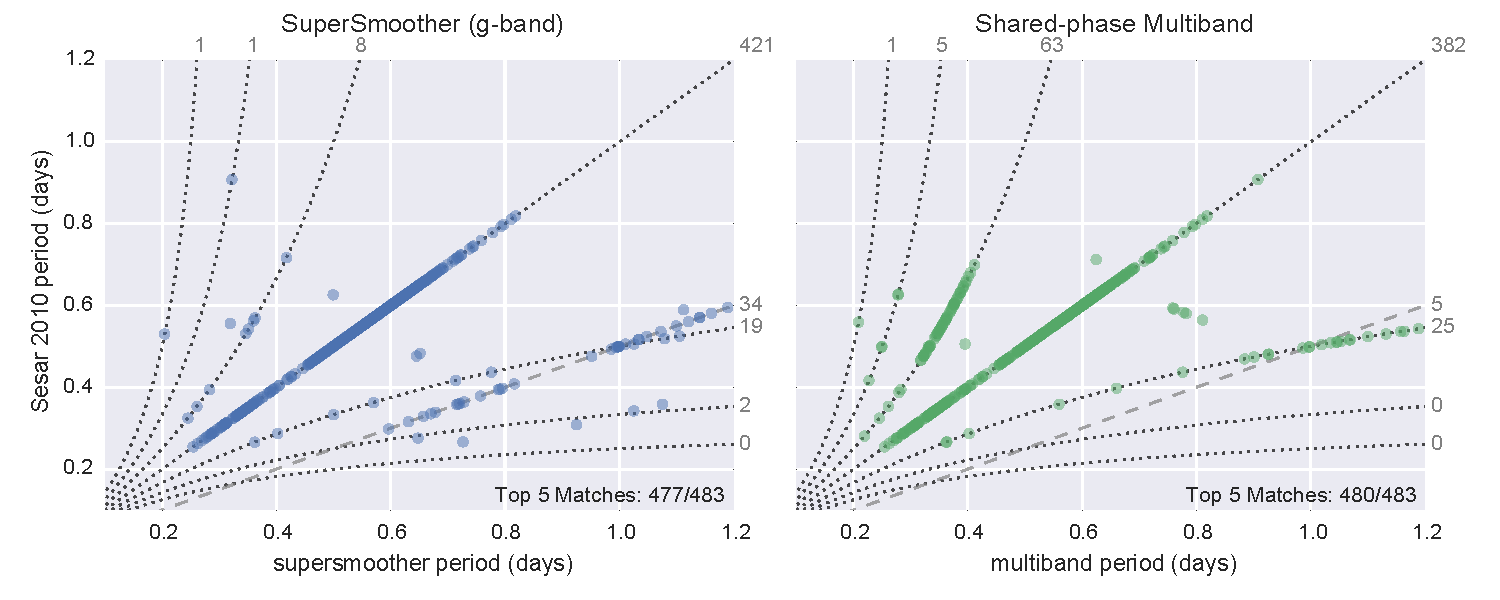
\includegraphics[width=\textwidth]{fig07b.pdf}
  \caption{
    Comparison of the Multiband algorithm and single-band supersmoother algorithm on 483 well-sampled RR Lyrae light curves from Stripe 82.
    The upper panels show a representative lightcurve and periodogram fits, while the bottom panels compare the derived periods to the true periods \citep[Based on a combined SuperSmoother and template-fitting approach; see][]{Sesar2010}.
    Shown for reference are the beat aliases (dotted lines) and the multiplicative alias (dashed line), along with counts of points aligned with each trend.
    The supersmoother algorithm tends to err toward multiplicative aliases, while the multiband algorithm tends to err toward beat frequency aliases.
    Both methods find the correct period among the top 5 significant peaks around 99\% of the time.
  } 
  \figlabel{compare_periods}
\end{figure}

The full S10 RR Lyrae dataset consists of 483 objects with an average of 55 observations in each of the five SDSS $ugriz$ bands spread over just under ten years.  In the upper panels of \fig{compare_periods} we show the observed data for one of these objects, along with the periodogram derived with the single-band supersmoother algorithm and the shared-phase $(0, 1)$-multiband algorithm\footnote{The supersmoother periodogram $P_{SS}$ is constructed from the minimum sum of weighted model residuals $\bar{r}_{min}$ in analogy with the Lomb-Scargle periodogram's $\chi^2$ interpretation from \eq{chi2PN}: $P_{SS}(\omega) = 1 - \bar{r}_{min}(\omega) / \bar{r}_0$}. Here we have a case which is analogous to that shown for simulated data in the top panels of \fig{multiband_sim}: each band has enough data to easily locate candidate peaks, the best of which is selected via the S10 template-fitting procedure.

The lower panels of \fig{compare_periods} compare the S10 period with the best periods obtained from the 1-band supersmoother (lower-left) and from the shared-phase multiband model (lower-right). To guide the eye, the figure includes indicators of the locations of beat aliases (dotted lines) and multiplicative aliases (dashed lines) of the S10 period.

The best-fit supersmoother period matches the S10 period in 89\% of cases (421/483), while the best-fit multiband period matches the S10 period in 79\% of cases (382/483). The modes of failure are instructive: when the supersmoother model misses the S10 period, it tends to land on a multiplicative alias. This is due to the flexibility of the supersmoother model: a doubled period spreads the points out further, leading to fewer constraints in each neighborhood and thus a smaller average residual around the over-fit model.  When the multiband model misses the S10 period, it tends to land on a beat alias between the S10 period and the 1-day observing cadence. This is due to the fact that the single-frequency periodic model significantly under-fits the data, and thus cannot distinguish deviations due to underfitting from deviations due to window function effects.

In both models, the S10 period appears among the top 5 periods 99\% of the time: $477/483$ for supersmoother, and $480/483$ for multiband.\footnote{We would expect this correspondence to be 100\% in the case of the $g$-band supersmoother, which was the model used in the first pass of the S10 computation. This discrepancy can be chalked-up to the different supersmoother implementations used in S10 and in this work. The discrepant curves are those with very low signal-to-noise.} This suggests that had S10 used the multiband Lomb-Scargle rather than the supersmoother in the first pass for that study, the final results presented there would be for the most part unchanged.

The results of this subsection show that the shared-phase multiband approach is comparable to the supersmoother approach for densely-sampled multiband data, although it has a tendency to get fooled by structure in the survey window function.

\subsection{Sparsely-sampled Multiband Data}

\begin{figure}
  \centering
  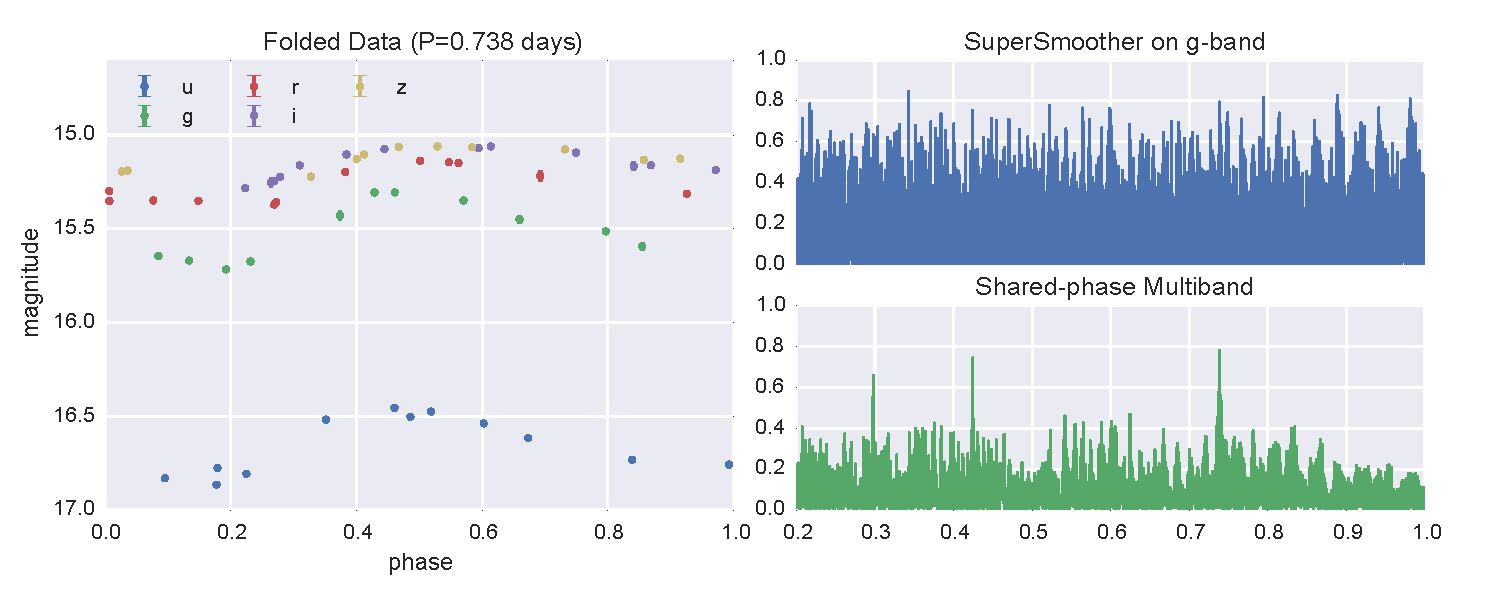
\includegraphics[width=\textwidth]{fig08a.pdf}
  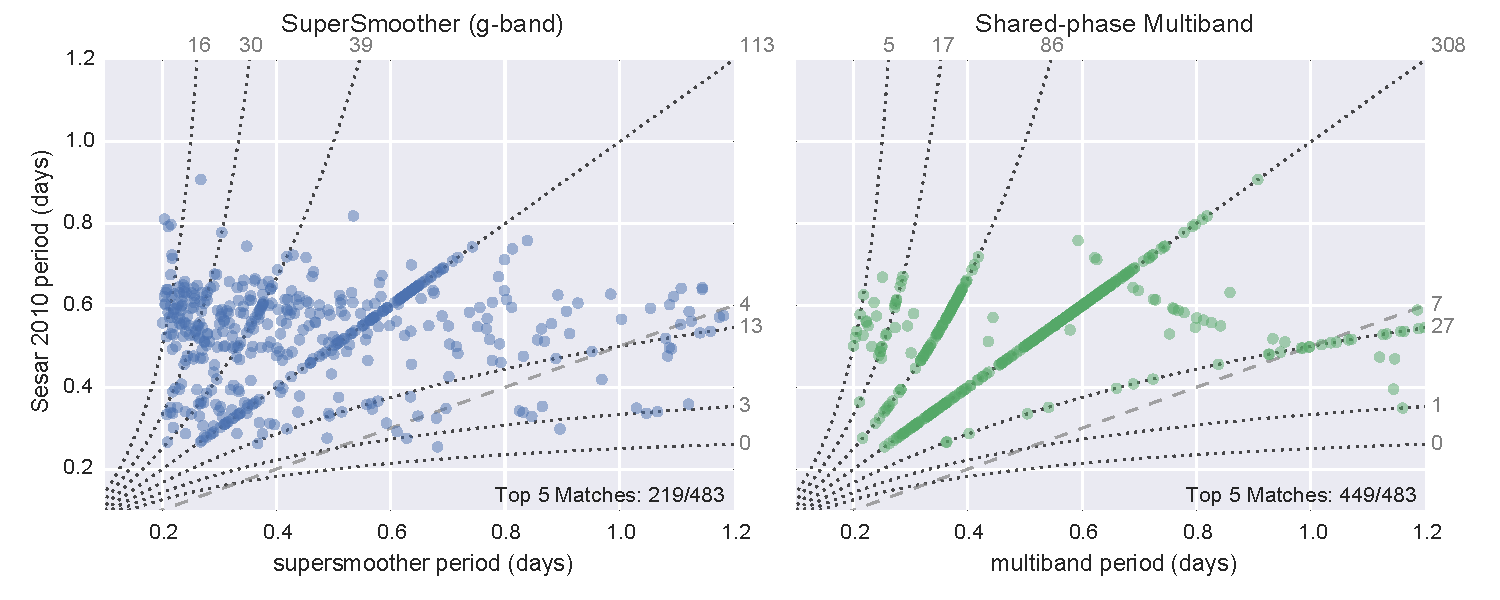
\includegraphics[width=\textwidth]{fig08b.pdf}
  \caption{
    This figure shows a repeat of the results from \fig{compare_periods}, but the data is artificially reduced to only a single-band observation on each evening, a situation reflective of the observing cadence of future large-scale surveys (compare to \fig{compare_periods}).
    In this case, the single-band SuperSmoother strategy used by \citet{Sesar2010} fails: there is simply not enough data in each band to recover an accurate period estimate, and the correct period is among the top 5 candidates in fewer than 60\% of cases.
    The shared-phase multiband approach utilizes information from all five bands, and returns much more robust results: even with the reduced data, the true period is among the top 5 candidates in 94\% of cases.
  } 
  \figlabel{compare_periods_reduced}
\end{figure}

Where we expect the multiband approach to have an advantage is when the data are sparsely sampled, with observations through only a single band each night. To simulate this, we reduce the Stripe 82 RR Lyrae dataset by a factor of 5, keeping only a single band of imaging each night, for an average of 11 observations of each object per band. This is much closer to the type of observation available in future multiband surveys.

The upper panels of \fig{compare_periods_reduced} show an example light curve from this reduced dataset, along with the supersmoother and multiband periodograms derived from this data. Analogously to the lower panels of \fig{multiband_sim}, the single-band supersmoother model loses the true period within the noise, while the shared-phase multiband model still shows a noticeable spike at this true period.

The lower panels of \fig{compare_periods_reduced} show the relationship between the S10 periods (based on the full dataset) and the periods derived with each model from this reduced dataset. It is clear that the supersmoother model is simply over-fitting noise with this few data points: the top period matches S10 in only 32\% of cases (compared to 87\% with the full dataset), and the top 5 periods contain the S10 period only 57\% of the time. The failure mode is much less regular as well: rather than being clustered near aliases, most of the points are scattered seemingly randomly around the space.

The multiband method does much better on the reduced dataset. Even with an 80\% reduction in the number of observations, the multiband method matches the S10 period 66\% of the time (compared to 79\% with the full dataset), and the top 5 periods contain the S10 period 94\% of the time. This performance is due to the fact that the multiband algorithm has relatively few parameters, but is yet able to accommodate data from multiple observing bands. In particular, this suggests that with the multiterm periodogram, the S10 analysis could have been done effectively with only a small fraction of the available data. This bodes well for future surveys, where data on variable stars will be much more sparsely sampled.

\section{Discussion and Conclusion}

\todo{Zeljko, can you take a stab at this?}

\begin{enumerate}
  \item Our method kicks ass, therefore we kick ass. QED.
  \item Future work: account for beat-aliases for ground-based data
  \item Future work: physically-motivated priors to further simplify the model
  \item Opportunity to apply this to PanSTARRS data release
\end{enumerate}


\bibliographystyle{apj}
\bibliography{paper}

\appendix
\section{{\tt multiband\_LS}: Python Implementation of Multiband Periodogram}
The algorithm outlined in this paper is available as an open-source Python package\footnote{\url{http://github.com/jakevdp/multiband_LS/}}, along with code to download the data and recreate all the figures in this paper.
{\tt multiband\_LS} is a pure-Python package written to be compatible with both Python 2 and Python 3, and performs fast numerical computation via the {\tt numpy} package\footnote{http://www.numpy.org}.

The API for the module is largely influenced by that of the {\tt scikit-learn} package\footnote{\url{http://scikit-learn.org}} \citep{scikit-learn}, in which models are class objects which can be ``fit()`` to data.
Here is a basic example of how you can use the code to download data, fit a multiband model to the data, and compute the power at a few periods:

\begin{lstlisting}
from multiband_LS import LombScargleMultiband

# Fetch the Sesar 2010 RR Lyrae data
from multiband_LS.data import fetch_light_curves
data = fetch_light_curves()
t, mag, dmag, filts = data.get_lightcurve(data.ids[0],
                                          return_1d=True)

# Construct the multiband model
model = LombScargleMultiband(Nterms_base=0, Nterms_band=1)
model.fit(t, mag, dmag, filts)

# Compute power at the following periods
model.periodogram([0.2, 0.3, 0.4])
\end{lstlisting}

Other models are available as well. For example, here is how you can compute the periodogram under the supersmoother model:

\begin{lstlisting}
from multiband_LS import SuperSmoother

# Construct the supersmoother model
model = SuperSmoother()
gband = (filts == 'g')
model.fit(t[gband], mag[gband], dmag[gband])

# Compute power at the following periods
model.periodogram([0.2, 0.3, 0.4])
\end{lstlisting}

The code contains many more methods, and much more functionality that what is shown here. For updates and more information, visit \url{http://github.com/jakevdp/multiband_LS}.

\end{document}
